\begin{subfigure}{.4\textwidth}
	\centering
	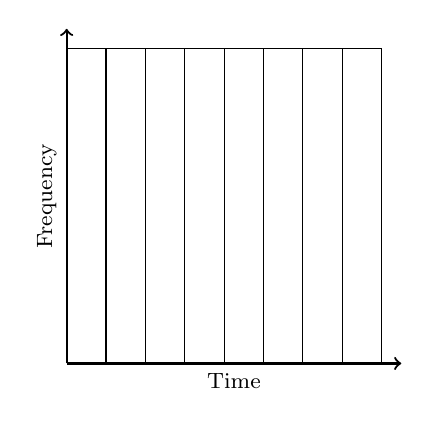
\begin{tikzpicture}
	\draw (0,0) -- (4,0);
	\draw (4,0) -- (4,-4);
	\path[thick, ->]  (0,-4) edge node[below] {\footnotesize Time} (4.25,-4)  ;
	\path[thick, ->] (0,-4) edge node[above, rotate=90] {\footnotesize Frequency} (0,.25)  ;
	
	\draw (.5,0) -- (.5,-4);
	\draw (1,0) -- (1,-4);
	\draw (1.5,0) -- (1.5,-4);
	\draw (2,0) -- (2,-4);
	\draw (2.5,0) -- (2.5,-4);
	\draw (3,0) -- (3,-4);
	\draw (3.5,0) -- (3.5,-4);
	\end{tikzpicture}
	\caption{Waveform}
\end{subfigure}%
\begin{subfigure}{.4\textwidth}
	\centering
	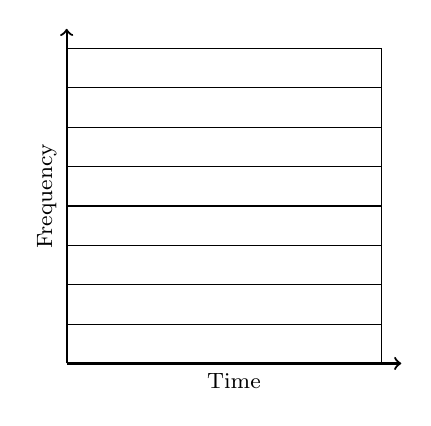
\begin{tikzpicture}
	\draw (0,0) -- (4,0);
	\draw (4,0) -- (4,-4);
	\path[thick, ->]  (0,-4) edge node[below] {\footnotesize Time} (4.25,-4)  ;
	\path[thick, ->] (0,-4) edge node[above, rotate=90] {\footnotesize Frequency} (0,.25)  ;
	
	\draw (0,-.5) -- (4,-.5);
	\draw (0,-1) -- (4,-1);
	\draw (0,-1.5) -- (4,-1.5);
	\draw (0,-2) -- (4,-2);
	\draw (0,-2.5) -- (4,-2.5);
	\draw (0,-3) -- (4,-3);
	\draw (0,-3.5) -- (4,-3.5);
	\end{tikzpicture}
	\caption{Fourier Transform}
\end{subfigure}

\medskip

\begin{subfigure}{.4\textwidth}
	\centering
		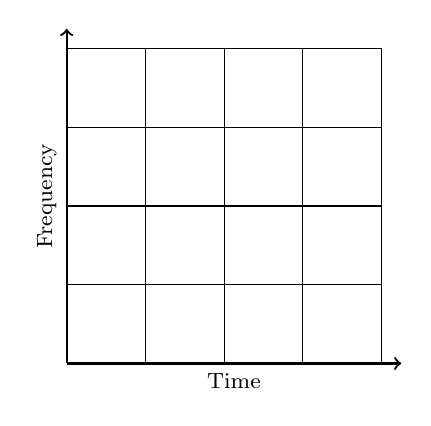
\begin{tikzpicture}
	
	\draw (0,0) -- (4,0);
	\draw (4,0) -- (4,-4);
	\path[thick, ->]  (0,-4) edge node[below] {\footnotesize Time} (4.25,-4)  ;
	\path[thick, ->] (0,-4) edge node[above, rotate=90] {\footnotesize Frequency} (0,.25)  ;
	
	\draw (1,0) -- (1,-4);
	\draw (0,-1) -- (4,-1);
	\draw (2,0) -- (2,-4);
	\draw (0,-2) -- (4,-2);
	\draw (3,0) -- (3,-4);
	\draw (0,-3) -- (4,-3);
	
	\end{tikzpicture}
	\caption{Short-Time Fourier Transform}
\end{subfigure}%
\begin{subfigure}{.4\textwidth}
	\centering
	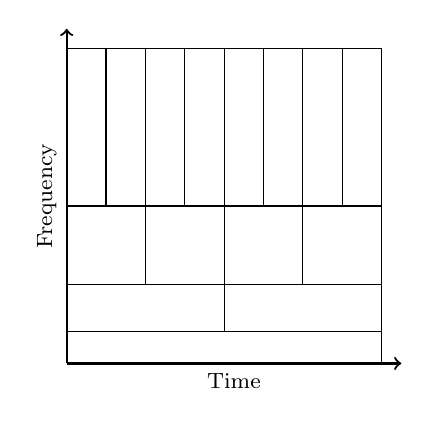
\begin{tikzpicture}
		\draw (0,0) -- (4,0);
		\draw (4,0) -- (4,-4);
		\path[thick, ->]  (0,-4) edge node[below] {\footnotesize Time} (4.25,-4)  ;
		\path[thick, ->] (0,-4) edge node[above, rotate=90] {\footnotesize Frequency} (0,.25)  ;
		\draw (0,-2) -- (4,-2);
		\draw (0,-3) -- (4,-3);
	
		\draw (0,-3.6) -- (4,-3.6);
		\draw (2,0) -- (2,-3.6);
	
		\draw[-] (1,0) -- (1,-3);
		\draw[-] (3,0) -- (3,-3);
	
		\draw[-] (.5,0) -- (.5,-2);
		\draw[-] (1.5,0) -- (1.5,-2);
	
		\draw[-] (2.5,0) -- (2.5,-2);
		\draw[-] (3.5,0) -- (3.5,-2);
	\end{tikzpicture}
	\caption{Wavelet Transform}
\end{subfigure}